\documentclass[a4paper,11pt]{article}
\usepackage[top=2cm,bottom=2cm,outer=2cm,inner=2cm]{geometry}
\usepackage[utf8]{inputenc}
\usepackage[T1]{fontenc}
\usepackage[inline]{enumitem}
\usepackage{amsfonts}
\usepackage{amsmath}
\usepackage{graphicx}


\title{Real Analysis \\ Homework 2}
\author{Yueh-Chou Lee}
\date{\today}
\begin{document}
\maketitle
\begin{enumerate}

% %%%%%%%%%%%%%%%%%%%%%%%%%%%%%%%%%%%%%%%%%%%%%%%%%%%%%%%%%%%%%%%%%%%
% Ex3

	\item (Exercise 9.3)
		\begin{enumerate}

			\item Show that if $f \in L^p (\mathbb{R}^n)$ and $K \in L^{p'} (\mathbb{R}^n)$, $1 \leq p \leq \infty$, $1/p + 1/p' = 1$, then $f \ast K$ is bounded and continuous in $\mathbb{R}^n$.

			\item Sketch the (trapezoidal) graph of $\chi_I \ast \chi_J$ where $I$ and $J$ are one-dimensional intervals. Consider also the case when the two intervals are the same.

		\end{enumerate}
	% \newline
	\textit{\textbf {Proof.}}\\
		\begin{enumerate}

			\item
				By H$\ddot{\text{o}}$lder's inequality, we know that
					$$(f \ast K)(x) = \int_{\mathbb{R}^n} f(x) K(x-t) dt
					\leq \left( \int_{\mathbb{R}^n} \left( f(t) \right)^p \right)^{1/p} \left( \int_{\mathbb{R}^n} \left( K(x-t) \right)^{p'} \right)^{1/p'}
					= ||f||_p ||K||_{p'}$$
				$f \ast K$ is bounded since $f \in L^p (\mathbb{R}^n)$ and $K \in L^{p'} (\mathbb{R}^n)$.\\

				If $1 \leq p \leq \infty$, $\infty \geq p' \geq 1$, then
					$$\begin{aligned}
					\left| f \ast K(x + \epsilon) - f \ast K (x) \right|
					&= \left| \int_{\mathbb{R}^n} f(t) [K(x+\epsilon-t) - K(x-t)] dt \right|\\
					\text{By H$\ddot{\text{o}}$lder's inequality} \hspace{0.2cm}
					&\leq ||f||_p || K(x+\epsilon-t) - K(x-t) ||_{p'}
					\to 0
					\hspace{0.4cm} \text{as $\epsilon \to 0$}
					\end{aligned}$$
				Since $f \in L^p (\mathbb{R}^n)$ and $K \in L^{p'} (\mathbb{R}^n)$.\\

			\item
				Let $I = [i_1,i_2]$, $J = [j_1,j_2]$.
				$$\chi_I \ast \chi_J = \int_{\mathbb{R}^1} \chi_I (t) \chi_J (x-t) dt$$

				\begin{figure}[htp]
				    \begin{center}
			        		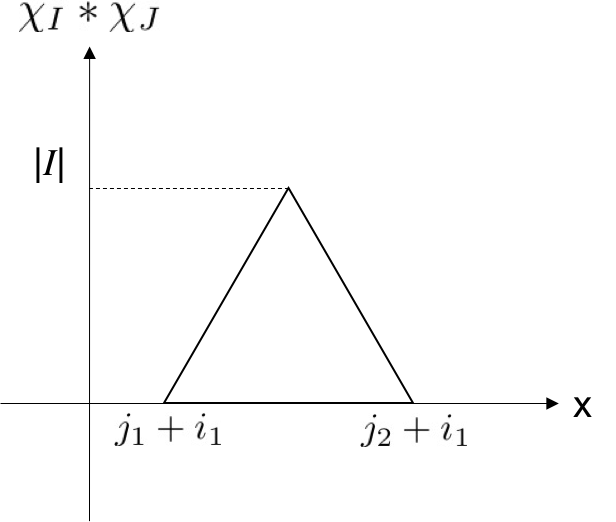
\includegraphics[scale=0.6]{9-3b}
				    \end{center}
				\end{figure}

		\end{enumerate}


% %%%%%%%%%%%%%%%%%%%%%%%%%%%%%%%%%%%%%%%%%%%%%%%%%%%%%%%%%%%%%%%%%%%
% Ex5
	\item (Exercise 9.5)\\
		Let $G$ and $G_1$ be bounded open subsets of $\mathbb{R}^n$ such that $\bar{G_1} \subset G$. Construct a function $h \in C_0^\infty$ such that $h = 1$ in $G_1$ and $h = 0$ outside $G$. (Choose an open $G_2$ such that $\bar{G_1} \subset G_2$, $\bar{G_2} \subset G$. Let $h = \chi_{G_2} \ast K$ for a $K \in C^\infty$ with suitably small support and $\int K = 1$.)\\
	\newline
	\textit{\textbf {Proof.}}\\
		Follow the hint, we can choose an open $G_2$ such that $\bar{G_1} \subset G_2 \subset \bar{G_2} \subset G$.\

		Define
			$$\begin{aligned}
			&\epsilon_1 = \inf \{ |x-y| : x \in G_1, y \in G_2^c \} = \text{dist} (G_1, \partial G_2)\\
			&\epsilon_2 = \inf \{ |x-y| : x \in G_2, y \in G^c \} = \text{dist}(G_2,\partial G)
			\end{aligned}$$
		and let $\epsilon = \min \{\epsilon_1, \epsilon_2 \}$.\

		By Exercise 9.4(c), we can choose $K \in C_0^\infty$ with $\text{supp}(K) = \overline{B_\epsilon (0)}$, so $K$ is integrable since $K$ is continuous with compact support.\

		Let $h = \chi_{G_2} \ast K$ for a $K \in C^\infty$ with suitably small support and $\int K = 1$. By Theorem 9.3, we know that $h \in C^\infty$ since $\chi_{G_2} \in L^1$ as $G_2$ is a bounded set.\

		If $x \in G_1$, then
			$$h(x)
			= \int_{\mathbb{R}^n} \chi_{G_2} (x - t) K(t) dt
			= \int_{B_\epsilon (0)} \chi_{G_2} (x - t) K(t) dt
			= \int_{B_\epsilon (0)} K(t) dt
			= 1$$
		since $x - t \in G_2$ for $|t| < \epsilon$.\

		If $x \in G^c$, then
			$$h(x)
			= \int_{\mathbb{R}^n} \chi_{G_2} (x - t) K(t) dt
			= \int_{B_\epsilon (0)} \chi_{G_2} (x - t) K(t) dt
			= 0$$
		since $x - t \notin G_2$ for $|t| < \epsilon$.\\

% %%%%%%%%%%%%%%%%%%%%%%%%%%%%%%%%%%%%%%%%%%%%%%%%%%%%%%%%%%%%%%%%%%%
% Ex7
	\item (Exercise 9.7)\\
		Let $f \in L^p (-\infty, +\infty)$, $1 \leq p \leq \infty$.  Show that the Poisson integral of $f$, $f(x, y)$, is harmonic in the upper half-plane $y > 0$.\\ (Show $((\partial^2/\partial x^2) + (\partial^2/\partial y^2)) f(x,y) = \int_{-\infty}^{+\infty} f(t) ((\partial^2/\partial x^2) + (\partial^2/\partial y^2)) P_y (x-t) dt$.)\\
	\newline
	\textit{\textbf {Proof.}}\\

		We say $f$ is harmonic on the upper half plane $y > 0$, if 
			$$\left( \frac{\partial^2}{\partial x^2} + \frac{\partial^2}{\partial y^2} \right) P_y (x) = 0$$
		Therefore, it suffices to show that
			$$\left( \frac{\partial^2}{\partial x^2} + \frac{\partial^2}{\partial y^2} \right) f(x,y)
			= \int_{-\infty}^{+\infty} f(t) \left( \frac{\partial^2}{\partial x^2} + \frac{\partial^2}{\partial y^2} \right) P_y (x-t) dt
			= 0$$
		Following, we will prove
			$$\frac{\partial}{\partial x} f(x,y)
			= \int_{-\infty}^{+\infty} f(t) \frac{\partial}{\partial x} P_y (x-t) dt$$
		Since $y > 0$, by definition
			$$\frac{\partial}{\partial x} P_y (x-t)
			= \underset{h \to 0}{\lim} \frac{P_y (x+h-t) - P_y(x-t)}{h}$$
		Let $\{h_n\}$ be a sequence tending to 0, $h_n \neq 0$, and define
			$$\phi_n (x,t) = \frac{P_y (x+h_n-t) - P_y(x-t)}{h_n}$$
		It follows that
			$$\frac{\partial}{\partial x} P_y (x-t) = \underset{n \to \infty}{\lim} \phi_n (x,t)$$
		Using Mean Value Theorem, we have
			$$|\phi_n (x,t)|
			\left| \frac{\partial}{\partial x} P_y (c-t) \right|
			\leq \underset{x \in \mathbb{R}}{\sup} \left| \frac{\partial}{\partial x} P_y (x-t) \right|$$
		for some $c \in (x, x+h_n)$.\

		Let $R > 0$ be arbitrary so that for $|x| \leq R$, we have
			$$\begin{aligned}
			\left| \frac{\partial}{\partial x} P_y (x-t) \right|
			&= \frac{1}{\pi} \left| \frac{\partial}{\partial x} \frac{y}{y^2 + (x - t)^2} \right|\\
			&= \frac{1}{\pi} \left| \frac{y}{y^2 + (x - t)^2} \cdot \frac{-2y (x - t)}{y^2 + (x - t)^2} \right|\\
			&\leq \frac{1}{\pi} \left( \frac{1}{y^2 + (x-t)^2} \right)\\
			&\leq \frac{1}{\pi} \frac{1}{y^2 + (\max \{ |t|-R,0 \})^2}\\
			&:= g(t)
			\end{aligned}$$
		Note that if $R$ is sufficiently large, for $|x| > R$, $\left| \frac{\partial}{\partial x} P_y (x-t) \right|$ is arbitrarily small since $\frac{1}{\pi} \left( \frac{1}{y^2 + (x-t)^2} \right)$ decays to 0 as $|x| \to \infty$.\

		Note that $g \in L^1(\mathbb{R}) \cap L^\infty (\mathbb{R})$. Next, note that $g \in L^1 (\mathbb{R}) \cap L^\infty (\mathbb{R})$ implies $g \in L^q (\mathbb{R})$, where $q$ is the H$\ddot{\text{o}}$lder conjugate of $p$.\
		Explanation: $\int |g|^q \leq ||g||_\infty^{q-1} \int |g| < \infty$.\

		Hence $||fg||_1 \leq ||f||_p ||g||_q < \infty$ by H$\ddot{\text{o}}$lder's inequality. Hence
			$$|f(t) \phi_n (x,t)| \leq |f(t) g(t)|$$
		where $fg$ is integrable.\

		Thus, by Lebesgue's Dominated Convergence Theorem, we know that
			$$\underset{n \to \infty}{\lim} \int_{-\infty}^{+\infty} f(t) \phi_n(x,t) dt
			= \int_{-\infty}^{+\infty} f(t) \underset{n \to \infty}{\lim} \phi_n(x,t) dt$$
		Since $y > 0$ and $R > 0$ are arbitrary,
			$$\frac{\partial}{\partial x} f(x,y)
			= \frac{\partial}{\partial x} \int_{-\infty}^{+\infty} f(y) P_y (x - t) dt
			= \int_{-\infty}^{+\infty} f(y) \frac{\partial}{\partial x} P_y (x - t) dt$$
		holds for the upper half-plane.\\

		Note that the main argument above is to find an integrable function that dominates $\left| f(t) \frac{\partial}{\partial x} P_y (x-t) \right|$.\

		Similarly, we can prove
			$$\frac{\partial^2}{\partial x^2} f(x,y)
			= \int_{-\infty}^{\infty} f(t) \frac{\partial^2}{\partial x^2} P_y (x,t) dt$$
		and the analogous statements for $\frac{\partial}{\partial y} f(x,y)$ and $\frac{\partial^2}{\partial y^2} f(x,y)$.\

		Briefly, since the Poisson kernel is smooth, all derivatives of it are bounded on all compact subsets of the upper half-plane. Furthermore, it decays to zero as $|x| \to \infty$, with faster decay for higher-order derivatives. Thus our dominating function $g(t)$ (multiplied by a constant) works for all derivatives.\\

% %%%%%%%%%%%%%%%%%%%%%%%%%%%%%%%%%%%%%%%%%%%%%%%%%%%%%%%%%%%%%%%%%%%
% Ex8
	\item (Exercise 9.8)\\
		(\textit{Schur's lemma}) For $s, t \geq 0$, let $K(s,t)$ satisfy $K \geq 0$ and $K(\lambda_s, \lambda_t) = \lambda^{-1} K(s,t)$ for all $\lambda > 0$, and suppose that $\int_0^\infty t^{-1/p} K(1,t) dt = \gamma < +\infty$ for some $p$, $1 \leq p \leq \infty$. For example, $K(s,t) = 1/(s+t)$ has these properties. Show that if
			$$(Tf)(s) = \int_0^\infty f(t) K(s,t) dt \hspace{0.4cm} (f \geq 0),$$
		then $||Tf||_p \leq \gamma ||f||_p$. (Note that $K(s,t) = s^{-1} K(1, t/s)$, and therefore $(Tf)(s) = \int_0^\infty f(ts)K(1,t) dt$. Now apply Minkowski's integral inequality [see Exercise 8 of Chapter 8].)\\
	\newline
	\textit{\textbf {Proof.}}\\

		Since
			$$(Tf) (s)
			= \int_0^\infty f(t) K(s,t) dt
			= \int_0^\infty f(t) K(1,t/s) dt/s
			= \int_0^\infty f(su) K(1,u) du$$
		If $1 \leq p < \infty$, then by Minkowski's integral inequality, we know that
			$$\begin{aligned}
			||Tf||_p
			& = \left( \int_{\mathbb{R}^n} | \int_0^\infty f(su) K(1,u) du|^p ds \right)^{1/p}\\
			& \leq \int_0^\infty \left( \int_{\mathbb{R}^n} |f(su) K(1,u)|^p ds \right)^{1/p} du\\
			& = \int_0^\infty \left( \int_{\mathbb{R}^n} |f(su)|^p d(su) \right)^{1/p} u^{-1/p} K(1,u) du\\
			& = ||f||_p  \int_0^\infty u^{-1/p} K(1,u) du\\
			& = \gamma ||f||_p
			\end{aligned}$$

		If $p = \infty$, then
			$$||Tf(s)||_\infty
			= \text{ess} \sup \left| \int_0^\infty f(su) K(1,u) du \right|
			\leq ||f||_\infty \left| \int_0^\infty K(1,u) du \right|
			= \gamma ||f||_\infty$$


% %%%%%%%%%%%%%%%%%%%%%%%%%%%%%%%%%%%%%%%%%%%%%%%%%%%%%%%%%%%%%%%%%%%
% Ex11
	\item (Exercise 9.11)\\
		Generalize Theorem 9.6 as follows: Let $f_\epsilon = f \ast K_\epsilon$, $K \in L^1(\mathbb{R}^n)$ and $\int_{\mathbb{R}^n} K = \gamma$. If $f \in L^p(\mathbb{R}^n)$, $1 \leq p < \infty$, show that $||f_\epsilon - \gamma f||_p \to 0$. Derive analogous results for Theorems 9.8, 9.9, and 9.13. (The case $\gamma \neq 0$ follows from the case $\gamma = 1$ by considering $K(x)/\gamma$.))\\
	\newline
	\textit{\textbf {Proof.}}\\

		If $\gamma \neq 0$. Let $g(x) = \frac{K(x)}{\gamma}$, then $g \in L^1(\mathbb{R}^n)$ and $\int_{\mathbb{R}^n} g = 1$.\\
		Let $g_\epsilon (x) = \epsilon^{-n} g(\frac{x}{\epsilon})$, then by Theorem 9.6, we know that
			$$||f_\epsilon - \gamma f||_p
			= ||f \ast K_\epsilon - \gamma f||_p
			= |\gamma| \cdot ||f \ast g_\epsilon - f||_p
			\to 0 \hspace{0.4cm} \text{as $\epsilon \to 0$}$$

		If $\gamma = 0$. Let $h \in L^1(\mathbb{R}^n)$ and $\int_{\mathbb{R}^n} h = 1$, then $K + h \in L^1(\mathbb{R}^n)$ and $\int_{\mathbb{R}^n} (K + h) = 1$.\\
		Let $h_\epsilon (x) = \epsilon^{-n} h(\frac{x}{\epsilon})$, then by Theorem 9.6, we know that
			$$\begin{aligned}
			||f_\epsilon - \gamma f||_p
			&= ||f \ast K_\epsilon ||_p\\
			&= ||f \ast (K_\epsilon + h_\epsilon) - f + f - f \ast h_\epsilon ||_p\\
			&\leq ||f \ast (K_\epsilon + h_\epsilon) - f||_p + || f - f \ast h_\epsilon ||_p
			\hspace{0.4 cm} \text{as $\epsilon \to 0$}
			\end{aligned}$$

		Analogous results for Theorems 9.8, 9.9 and 9.13 can be obtained by replacing $f_\epsilon \to f$ by $f_\epsilon \to \gamma f$ as $\epsilon \to 0$.\\

% %%%%%%%%%%%%%%%%%%%%%%%%%%%%%%%%%%%%%%%%%%%%%%%%%%%%%%%%%%%%%%%%%%%
% Ex12
	\item (Exercise 9.12)\\
		Show that the conclusions of Theorems 9.9 and 9.13 remain true if the assumption that $f \in L^1$ is replaced by $f \in L^p$, $p > 1$.\\
	\newline
	\textit{\textbf {Proof.}}\\

	\begin{enumerate}
		\item [(Theorem 9.9)]

			If $f$ is continuous at $x$, then given $\lambda > 0$, choose $\delta > 0$ such that $|f(x-t) - f(x)| < \lambda$ if $|t| < \delta$.
				$$\begin{aligned}
				|f_\epsilon (x) - f(x)|
				&= |\int_{\mathbb{R}^n} (f(x-t) - f(x)) K_\epsilon (t) dt|\\
				&\leq \lambda ||K||_1 + |f(x)| \int_{|t| \geq \delta} |K_\epsilon (t)| dt + \int_{|t| \geq \delta} |f(x-t)| |K_\epsilon (t)| dt
				\end{aligned}$$

			$|f(x)| \int_{|t| \geq \delta} |K_\epsilon (t)| dt \to 0$ as $\epsilon \to 0$.\

			Since $K(x) = o(|x|^{-n})$, $h(x) = \frac{K(x)}{|x|^{-n}} \to 0$ as $|x| \to \infty$, i.e. $K(x) = |x|^{-n} h(x)$.\

			Hence
				$$\begin{aligned}
				\int_{|t| \geq \delta} |f(x-t)| |K_\epsilon (t)| dt
				&= \int_{|t| \geq \delta} |f(x-t)| |t|^{-n} |h(\frac{t}{\epsilon})| dt\\
				&\leq \delta^{-n} \underset{|t| \geq \delta}{\sup} |h(\frac{t}{\epsilon})| \int_{|t| \geq \delta} |f(x-t)| dt\\
				\text{By H$\ddot{\text{o}}$lder's inequality} \hspace{0.2cm}
				&\leq \delta^{-n} \underset{|t| \geq \delta}{\sup} |h(\frac{t}{\epsilon})| ||f||_p ||1||_{\frac{p}{p-1}}\\
				&= \delta^{-n} \underset{|t| \geq \delta}{\sup} |h(\frac{t}{\epsilon})| ||f||_p \to 0
				\hspace{0.5cm} \text{as $\epsilon \to 0^+$}
				\end{aligned}$$

			So the conclusion of Theorem 9.9 remains true.\\

		\item [(Theorem 9.13)]
			The proof is similar with the proof in the textbook, we can change the conculsion of Theorem 9.9 that they used in the Theorem 9.13 to the above one. Then the conclusion of Theorem 9.13 will also remain true.\\
	\end{enumerate}

% %%%%%%%%%%%%%%%%%%%%%%%%%%%%%%%%%%%%%%%%%%%%%%%%%%%%%%%%%%%%%%%%%%%
% Ex13
	\item (Exercise 9.13)\\ 
		Let $f \in L^p(0,1)$, $1 \leq p \leq \infty$, and for each $k = 1,2,...,$ define a function $f_k$ on $(0,1)$ by letting $I_{k,j} = \{x : (j-1) 2^{-k} \leq x \leq j 2^{-k} \}$, $j = 1,...,2^k$, and setting $f_k(x)$ equal to $|I_{k,j}|^{-1} \int_{I_{k,j}} f$ for $x \in I_{k,j}$. Prove that $f_k \to f$ in $L^p(0,1)$ norm. (Exercise 17 of Chapter 7 may be helpful for the case $p = 1$.)\\
	\newline
	\textit{\textbf {Proof.}}\\

		Note that $|I_{k,j}|^{-1} = 2^k$, and
			$$f_k (x) = \sum_{j=1}^{2^k} 2^k \int_{I_{k,j}} f(t) dt \chi_{I_{k,j}} (x)$$
		Then we will prove that $f_k \in L^p (0,1)$ for all $k \in \mathbb{N}$.
			$$\begin{aligned}
			\int_0^1 |f_k(x)|^p dx
			&= \int_0^1 \left| \sum_{j=1}^{2^k} 2^k \int_{I_{k,j}} f(t) dt \chi_{I_{k,j}} (x) \right|^p dx\\
			&= 2^{kp} \sum_{j=1}^{2^k} \int_{I_{k,j}} \left| \int_{I_{k,j}} f(t) dt \right|^p dx\\
			&\leq 2^{kp} \sum_{j=1}^{2^k} \int_{I_{k,j}} \left[ \int_{I_{k,j}} |f(t)| dt \right]^p dx\\
			\text{By H$\ddot{\text{o}}$lder's inequality} \hspace{0.2cm}
			&\leq 2^{kp} \sum_{j=1}^{2^k} \int_{I_{k,j}} \left[ \left( \int_{I_{k,j}} |f(t)|^p dt \right)^{1/p} \left( \int_{I_{k,j}} |1|^{p'} dt \right)^{1/p'} \right]^p dx\\
			&= 2^{kp} \sum_{j=1}^{2^k} \int_{I_{k,j}} \left[ \left( \int_{I_{k,j}} |f(t)|^p dt \right) 2^{-kp/p'} \right] dx\\
			&= 2^{kp - k - kp/p'} \sum_{j=1}^{2^k} \int_{I_{k,j}} |f(t)|^p dt\\
			&= \int_)^1 |f(t)|^p dt\\
			&= ||f||_p^p < \infty
			\end{aligned}$$

		By Lebesgue’s Differentiation Theorem, $f_k \to f$ a.e. By Fatou’s Lemma, we have
			$$\int_0^1 |f|^p
			\leq \lim \text{inf} \int_0^1 |f_k|^p
			\leq \lim \text{sup} \int_0^1 |f_k|^p
			\leq \int_0^1 |f|^p$$
		Hence $||f_k||_p \to ||f||_p$.\

		Follow the hint, by using Exercise 8.12, we know that if $f_k \to f$ a.e. and $||f_k||_p \to ||f||_p$, $0 < p < \infty$, then $||f - f_k||_p \to 0$, so we can conclude that $f_k \to f$ in $L^p(0,1)$ norm.\\



\end{enumerate}
\end{document}